\chapter{Steady state heat transfer in solids}
\label{ch:heatcases1}

\section{Concept map}

\index{Concept map, heat transfer solutions}

\begin{figure}[h]
\begin{center}
\framebox{
\includegraphics[scale=0.5]{images/c16-HeatTransferConceptMap.eps}
}
\end{center}
\caption{Concept map on heat transfer solutions}
\label{conceptmapheatsolutions}
\end{figure}


\section{Steady state 1D heat transfer}

\subsection{Across a rectangular slab}

\begin{figure}[h]
\begin{center}
\framebox{ 
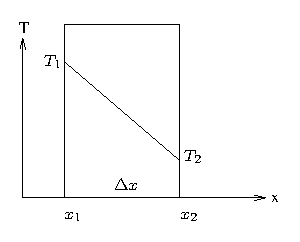
\includegraphics[scale=0.7]{images/c16-slabfig.ps}
}
\end{center}
\caption{Heat flow across a slab}
\label{slab}
\end{figure}

At steady state, if $q$ is the rate of heat transfer ($Js^{-1}$) across a slab
area $A$:

$$ \frac{q}{A} = -k \frac{\partial T}{\partial x} $$

If the surface temperatures of the slab are $T_1$ and $T_2$ at $x_1$ and $x_2$,
respectively, then:

$$ \int_{T_1}^{T_2}{dT} = \frac{-q}{Ak} \int_{x_1}^{x_2}{dx} $$

$$ T_2 - T_1 = \frac{q}{Ak} (x_1 - x_2) = - \frac{q}{Ak} \Delta x $$

\begin{equation}
\boxed{
  \frac{T_1 - T_2}{q} = \frac{\Delta x}{Ak}
}
\end{equation}

Taking the analogy of electricity, $T_1 - T_2$ is the driving force similar to
voltage, $q$ is the flux similar to current and $\frac{\Delta x}{Ak}$ is the
resistance. Now the resistance to heat flow is known, they can combined in
serial and parallel similar to the circuits in electricity.

As can be seen from the equation for flux:
$$\frac{q}{A} = k \frac{T_1 - T_2}{\Delta x}$$
doubling the slab thickness $\Delta x$ will halve the heat flux.

We can write the heat flux at the inner wall as follows:

\begin{equation}
	\left. \frac{q}{A} \right|_{1} = \left( k \frac{\Delta T}{\Delta x} \right) \, f 
\end{equation}

Here, the geometric factor $f$ is equal to unity for planar shells.

\subsection{Across a cylindrical wall} 

\begin{figure}[h]
\begin{center}
\framebox{
 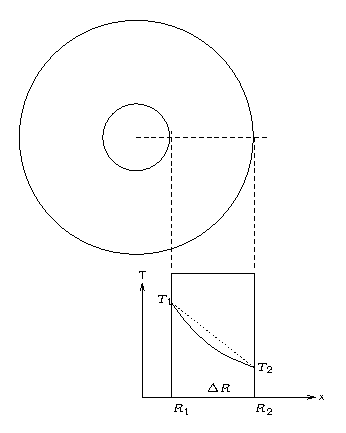
\includegraphics[scale=0.7]{images/c16-cylwallfig.ps}
}
\end{center}
\caption{Heat flow across a cylindrical wall}
\label{cylwall}
\end{figure}

At steady state, if $q$ is the rate of heat transfer ($Js^{-1}$) across a
cylindrical wall of (variable) area $A=2\pi r L$:

$$ \frac{q}{A} = \frac{q}{2\pi r L} = -k \frac{\partial T}{\partial r} $$

Heat flow across a hollow cylindrical wall of inner radius $R_1$ and outer $R_2$
at temperatures $T_1$ and $T_2$, respectively, is then given by:

$$ \int_{T_1}^{T_2}{dT} = \frac{-q}{2\pi L k} \int_{R_1}^{R_2}{\frac{dr}{r}}$$

$$ T_2 - T_1 = \frac{-q}{2\pi L k} \ln{\frac{R_2}{R_1}}$$

\begin{equation}
\boxed{
  \frac{T_1 - T_2}{q} = \frac{ \ln{\frac{R_2}{R_1}} } {2\pi L k}
}
\end{equation}

Drawing the analogy to electricity as above, the resistance to heat flow across
a cylindrical wall is $\frac{\ln{\frac{R_2}{R_1} }} {2\pi L k}$.

As can be seen from the equation for flux:
$$\frac{q}{A}|_{r=R_1} = \frac{q}{2\pi L R_1} = k \frac{T_1 - T_2}{R_1
\ln{\frac{R_2}{R_1}}} = k \frac{T_1 - T_2}{R_1 \ln{(1+ \frac{\Delta R}{R_1})}}
$$

Doubling the slab thickness $\Delta R$ will \textit{not necessarily} halve the
heat flux. It can be noted that in the limit of large curvature, $R_1
\rightarrow \infty$, $\frac{\Delta R}{R_1}$ is a small quantity and $\ln{(1+
\frac{\Delta R}{R_1})}$ can be approximated to $\frac{\Delta R}{R_1}$ leading to
the above expression as:

$$\frac{q}{A}|_{r=R_1 \rightarrow \infty} = k \frac{T_1 - T_2}{R_1 \frac{\Delta
R}{R_1}} = k \frac{T_1 - T_2}{ \Delta R} $$

which is the limit where a cylindrical wall of thickness $\Delta R$ can be
approximated to a rectangular slab of same thickness.

We can write the heat flux at the inner wall as follows:

\begin{equation}
	\left. \frac{q}{A} \right|_{1} = \left( k \frac{\Delta T}{\Delta R} \right) \, f 
\end{equation}

Here, the geometric factor $f$ for cylindrical shell is written as:

\begin{equation}
	f = \frac{ \frac{\Delta R}{R_1}}{\ln\left(1 + \frac{\Delta R}{R_1}\right)}
\end{equation}


\subsection{Across a spherical shell}

At steady state, if $q$ is the rate of heat transfer ($Js^{-1}$) across a
spherical shell of (variable) area $A=4\pi r^2$:

$$ \frac{q}{A} = \frac{q}{4\pi r^2} = -k \frac{\partial T}{\partial r} $$

Heat flow across a hollow sphere of inner radius $R_1$ and outer $R_2$ at
temperatures $T_1$ and $T_2$, respectively, is then given by:

$$ \int_{T_1}^{T_2}{dT} = \frac{-q}{4\pi k} \int_{R_1}^{R_2}{\frac{dr}{r^2}}$$

$$ T_2 - T_1 = \frac{-q}{4\pi k} \left( \frac{1}{R_1} - \frac{1}{R_2} \right) $$

\begin{equation}
\boxed{
  \frac{T_1 - T_2}{q} = \frac{1}{4\pi k} \left( \frac{1}{R_1} - \frac{1}{R_2}
\right)
}
\end{equation}

Drawing the analogy to electricity as above, the resistance to heat flow across
a cylindrical wall is $\frac{1}{4\pi k} \left( \frac{1}{R_2} - \frac{1}{R_1}
\right)$.

$$\left. \frac{q}{A} \right|_{r=R_1 \rightarrow \infty} =  k \frac{(T_1 -
T_2)R_2}{\Delta R R_1} = \left. k \frac{T_1 - T_2}{\Delta R} \left( 1 + {\Delta
R \over R_1}\right) \right|_{R_1 \rightarrow \infty} = k {T_1 - T_2 \over \Delta
R}$$

which is the limit where a spherical shell of thickness $\Delta R$ can be
approximated to a rectangular slab of same thickness.

We can write the heat flux at the inner wall as follows:

\begin{equation}
	\left. \frac{q}{A} \right|_{1} = \left( k \frac{\Delta T}{\Delta R} \right) \, f 
\end{equation}

Here, the geometric factor $f$ for spherical shell is written as:

\begin{equation}
	f = \left(1 + \frac{\Delta R}{R_1} \right)
\end{equation}


\subsection{Point effect of diffusion}

When the temperature differences and the properties are kept constant, heat flux
(heat per unit time per unit area) depends on the geometry - with the following
geometries in the decreasing order of effectiveness: point, line, plane, edge,
corner. Such a sequence of effectiveness of thermal diffusion arises from the
amount of space available for exchange of energy. Point effect of diffusion comes of use when interpreting defects in casting.

As can be seen from the equation for flux:

Doubling the slab thickness $\Delta R$ will \textit{not necessarily} halve the
heat flux. It can be noted that in the limit of large curvature, $R_1
\rightarrow \infty$, $\frac{\Delta R}{R_1}$ is a small quantity and goes to zero
leading to the above expression as:

$$\left. \frac{q}{A}\right|_{r=R_1 \rightarrow \infty} = k \frac{T_1 -
T_2}{\Delta R} $$

which is the limit where a spherical wall of thickness $\Delta R$ can be
approximated to a slab of same thickness.

The rationale behind this is the what we call as \textit{point effect of
diffusion}. Taking the wall thickness to be same, we plot the three geometries
below: 

\begin{figure}[h]
\begin{center}
\framebox{
 \includegraphics[scale=0.7]{images/c16-pediff.eps}
}
\end{center}
\caption{Point effect of diffusion}
\label{pediff}
\end{figure}


\subsection{Across a planar composite wall}

Using the electrical analogy of the previous section, flux boundary condition
$\frac{q}{A} = h \left(T_s - T_\infty \right)$ can be written such that the
resistance to heat flow is $\frac{1}{Ah}$.

At steady state, if $q$ is the rate of heat transfer ($Js^{-1}$) across a planar
composite wall of constant area $A$:

$$ \frac{q}{A} = h_b \left(T_b - T_1 \right) = 
      -k_{12} \frac{T_2 - T_1}{\Delta x_{12}} = 
      -k_{23} \frac{T_3 - T_2}{\Delta x_{23}} = 
      -k_{34} \frac{T_4 - T_3}{\Delta x_{34}} = 
       h_a \left(T_4 - T_a \right) $$

or

$$ T_a - T_b = \frac{q}{A} \left[ \frac{1}{h_a} + 
                                  \frac{\Delta x_{12}}{k_{12}} +
                                  \frac{\Delta x_{23}}{k_{23}} +
                                  \frac{\Delta x_{34}}{k_{34}} +
                                  \frac{1}{h_b} \right] $$

Analogy with electricity: $\frac{1}{h}$ and $\frac{\Delta x}{k}$ act as
resistances. Temperature is analogous to voltage difference (driving force for
the current). $\frac{q}{A}$ is analogous to current.

\subsection{Across a cylindrical composite wall}

Using the electrical analogue of the previous section, the heat flow across a
composite hollow cylindrical wall is given by:

$$ T_a - T_b = \frac{q}{2 \pi L} \left[ \frac{1}{r_1 h_1} +
\frac{\ln{\frac{r_1}{r_2}}}{k_{12}} + \frac{\ln{\frac{r_2}{r_3}}}{k_{23}} +
\frac{\ln{\frac{r_3}{r_4}}}{k_{34}} + \frac{1}{r_4 h_4} \right] $$

\pagebreak
\section{Exercises}

\begin{enumerate}

 \item Heat is flowing at steady state through an annular wall of a cylinder of
inner radius $R_1$ and outer radius $R_2$. Thermal conductivity of the wall
material is approximated to be linear function of temperature with a value of
$k_1$ at the inner wall temperature $T_1$ and $k_2$ at the outer wall
temperature $T_2$. (a) Derive an expression for the heat flow across the
cylindrical shell. (b) Simplify the expression for the case when the wall
thickness is very small compared to the radius of the cylinder.


 \item Example 6.3 of~\cite{gaskell}. Hot water flows through a glass tube of
inner radius \SI{3}{\cm} and outer radius \SI{5}{\cm}. The temperatures of the
inner and outer surfaces of the tube are, respectively, \SI{90}{\celsius} and
\SI{85}{\celsius} and the mean thermal conductivity of the glass is
\SI{0.84}{\wpmk} . (a) Calculate the rate of heat loss from the tube per unit
length. (b)By how much is the rate of heat loss decreased if the wall thickness
of the tube is doubled keeping the inner radius same.\\ {\bf Answer:} (a)
\SI{51.7}{\watt\per\metre} (b) \SI{31.1}{\watt\per\metre}

 \item An iron slab of thickness \SI{2}{\cm} carries an electric current that
generates heat at a rate of \SI{10e6}{\watt\per\metre\cubed}. If the right side
face of the slab is at \SI{20}{\celsius}, what should be the temperature of the
left side face such that all the heat flux in the slab is from the left face to
the right face at steady state? Properties of steel are $k$ = \SI{45}{\wpmk},
$\rho$ = \SI{7210}{\kgpmc} and $C_p$ =
\SI{750}{\joule\per\kilo\gram\per\kelvin}.

\item Example 6.4 of~\cite{gaskell}. A furnace wall consists of \SI{15}{
		\centi\metre} thick silica brick ($k$ = \SI{1.1}{\wpmk}), a \SI{5}{\cm} glass
fibre ($k$ = \SI{0.035}{\wpmk} and a \SI{1}{\cm} steel ($k$ = \SI{45}{\wpmk}).
Inner temperature of the furnace is \SI{500}{\celsius} and heat transfer
coefficient on the inner wall is \SI{15}{\wpmsk}. Ambient temperature is
\SI{20}{\celsius} and heat transfer coefficient on the outer wall is
\SI{20}{\wpmsk}. (a) Calculate the power loss per unit area of furnace wall at
steady state. (b) Temperatures at each junction. \\ {\bf Answer:} (a)
		\SI{285.4}{\watt\per\metre\squared} (b) $T_i = $ \SI{481}{\celsius}, $T_1 = $ \SI{442}{
			\celsius}, $T_2 \approx T_3 \approx$ \SI{34}{\celsius}.

 \item A \SI{50}{\cm} long tubular furnace is made of a \SI{1}{\cm} thick silica
tube of \SI{10}{\cm} inner radius kept in a \SI{5}{\mm} thick steel tube of
\SI{15}{\cm} outer dia with glass wool in between. Knowing that the glass wool
would melt at \SI{800}{\celsius} and that furnace converts all its electrical
power to heat energy, (a) what is the highest temperature that can be set in the
furnace and (b) what is the power consumption at that temperature setting? 
Ignore end effects and assume steady state. The heat transfer coefficients for
inside and outside of the furnace can be taken to be \SI{20}{\wpmsk}. Assume
room temperature to be \SI{300}{\kelvin} .


 \item Example 6.7 of~\cite{gaskell}. A copper wire of diameter \SI{1}{
		 \milli\metre} has an insulating plastic sheath of \SI{0.5}{\mm} around it. The
heat transfer coefficient on the surface exposed to ambient air at
\SI{30}{\celsius} is \SI{8}{\wpmsk}. If the insulating plastic softens above
\SI{100}{\celsius}, calculate the maximum current that can be passed through the
wire. Properties of copper are $k$ = \SI{380}{\wpmk}, $\sigma$ =
\SI{1.96e-8}{\ohm\metre}. Properties of the insulating plastic are $k$ =
		\SI{0.35}{\wpmk} and $\sigma \approx \SI{0}{\ohm\metre}$. \\ {\bf Answer:} \SI{14.3}{
			\ampere}
\end{enumerate}

% ----------------------- end of heatcases1.tex --------------------
